%----------------------------------------------------------------------------
\chapter{Summary, conclusions}
%----------------------------------------------------------------------------
\begingroup
\setlength{\intextsep}{0pt}%
\setlength{\columnsep}{10pt}%
\begin{wrapfigure}[16]{r}{60mm}
\vspace{-90pt}
\begin{center}
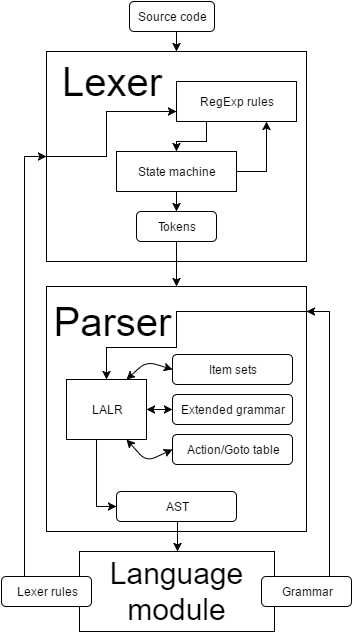
\includegraphics[width=60mm,keepaspectratio]{figures/diagram.png}
\end{center}
\vspace{-15pt}
\caption{High level architectural overview}
\end{wrapfigure}

The original goal of this thesis was to create a usable parser module in JavaScript that is as easy to use as to understand. Since my background in formal languages was limited, I aimed to use an algorithm that I could completely understand. This is the reason behind my first solution --- I tried to solve the problem using only intuition, to see what can be done without previous knowledge of the subject.

While this turned out to be somewhat of a waste of time, I did learn a lot from this failure. I had a better grasp at what has to be done, and I was eager to find out how a proper solution worked. This lead me to choose one of the state-machine based algorithms, and to eliminate the left-recursion problem, I ended up looking at LR parsers. I decided to use the LALR parser algorithm because of it being a bit more memory efficient, and not the easiest to implement --- but not the hardest either.

While creating an implementation for the steps of LALR parser construction, I tried to use algorithms that are easy to understand, so that others can build upon and understand my solution later.

The two examples show how easy it is to run code in any custom language in the browser with this modular interpreter --- and how easy it is to write modules for languages. This satisfies the initial goal of making the creation of educational websites easier. For example using this parser, HTML based presentations could be built for programming classes that have live demo codes on the slides that can be modified even during presentation. In the more traditional sense, simple programming education websites could use this interpreter to provide a simple programming environment to the students, keeping them close to the learning material.

The source code of the solution is available on GitHub in a public repository (\url{https://github.com/brenca/szakdolgozat}). This thesis is also available in the repository, since it serves as a detailed documentation for the solution. 
\endgroup